\documentclass[a4paper,12pt,line]{article}
% importing all the necessary packages before getting begin the document
\usepackage{color}
\usepackage{graphicx}
\usepackage[top=0in, bottom=0in, left=0.35in, right=0.85in]{geometry}
\usepackage{tikz}
\usepackage{tabularx}
\usepackage{hyperref}
\usepackage{colortbl}
\pagecolor{yellow!0}
\color{black}
\definecolor{rd}{RGB}{255,127,37}%manually defining a colour by giving RGB values
\pagestyle{empty}
\setlength{\parindent}{10ex}
\renewcommand{\baselinestretch}{1.5}


%initialising a document
\begin{document}
	
	%---------------------------- #1 ---------------------%
	%initialising space for creation of Top Red colour border>This is the theme of the Resume
	%-----------by drawing a rectangle filled with predefined color
	%using hspace to make the rectange to fit perfectly at the head of document
	\hspace*{-19mm}
	
\begin{tikzpicture}
		\draw [fill=rd,rd] (0,0) rectangle (19.4,0.5);
	\end{tikzpicture}
	\vspace*{3pt}
	
	
	%---------------------------- #2 ---------------------%
	%Name -- using color and Huge,LARGE size fonts and Bolded type of text
	%First name with full darkness in colour and Sur name at level 60 darkness
	%This is to differentiate The First name and Last name
	\begin{center}
		{\color{magenta}\Huge{\textbf{N}}\LARGE\textbf{\textrm{ISHANTH}}}\\
		\vspace{13pt}	
		{\color{magenta!60}\hspace{.8cm}\Huge{S}\LARGE\textsc{HANMUGAM}}\\
	\end{center}
	\vspace*{13pt}
	
	%---------------------------- #3 ---------------------%
	% Permanant address and contact information
	%Using flush left to allign the address to the left margin of the page
	%
	%-----Inserting profile pic at the declared location ,say (put(420,230))
	%and adjusting the width of the pic
	%
	%The pic should be stored in the location of this Program
	\begin{flushleft}
		5/309,	
		Rajiv gandhi nagar,\\
		Salem Road,\\
		Namakkal,\hspace{9.6cm}Mobile : +91-7200331572\\
		Tamilnadu.\hspace{9.5cm}E-mail : nishanthsnh@gmail.com\\
		
		\begin{picture}(0,0)
		\put(420,130){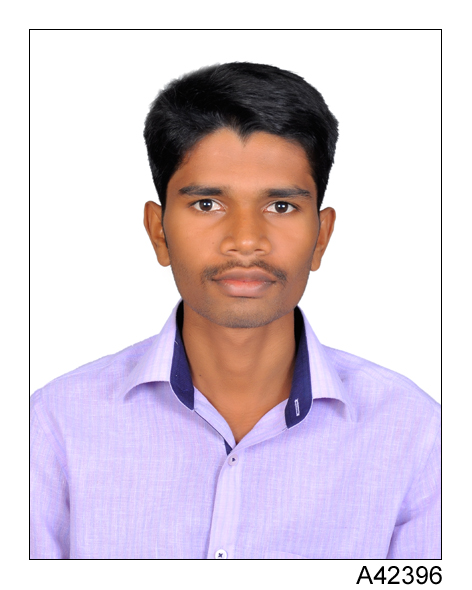
\includegraphics[width=30mm]{my.jpg}}
		\end{picture}
		
	\end{flushleft}
	\vspace{-15mm}

	%---------------------------- #4 ---------------------%
	%First section named as Objective with Magenta color
	\section*{\color{magenta}Objective}
	
		\hspace{10mm}To get and share my knowledge to the platform where I work, and to innovate an useful, service based idea for the growth of my Nation as well as my workplace
		
		
	%---------------------------- #5 ---------------------%
	
	%Initiation of table of 5 columns centered text with out vertical line
	%Colouring the row for highliting using colortbl package
	\section*{\color{magenta}Education}
	\begin{tabular}{ccccc}
		%\hline
		\rowcolor{yellow!20}
		\color{blue}\textsc{Degree}&\color{blue}\textsc{College/School}&\color{blue}\textsc{Board}&\color{blue}\textsc{Passing Year} &\color{blue}\textsc{Percentage}\\%\hline
		\rowcolor{orange!30}
		B.E(EIE)&M.Kumarasamy College of Engineering&Anna University&2017&8.1\textsuperscript{*}\\\rowcolor{orange!30}
		HSC&Bharathi higher secondary school&StateBoard&2013&86\\\rowcolor{orange!30}
		SSLC&Bharathi higher secondary school&StateBoard&2011&94\\
		
	\end{tabular}
	\begin{flushright}
		*upto 7th semester
	\end{flushright}
		
\end{document}